This discussion is structured into two semi-independent parts: We first summarize the results from the simulation study and reflect on how we can develop on the methods especially on the numerical optimization side. Furthermore, we mention two estimation methods that could be interesting to consider in future research.\\
Then we put the results from the estimation on the AMOC into perspective, contrasting it with previous findings. We add a robustness analysis to our findings in the same way  Here, we also discuss how one might go about selecting between models from \ref{table:ergodicDiffusions}. In particular, with our models as a starting point we discuss what type of role the stochastic part in these types of analysis can have. \\
Finally, we mention a couple of other ideas that can be used on these models in practice. In extension, we reflect on the different ways one can use models such as these more generally.
\subsection{Simulation studies}
Our starting point for the discussion is a short look into the results shown in figures \ref{figure:parameter_precision_dynamic} and \ref{figure:overviewOfEstimatorsStationary}. As we noted it is not given that the behaviour shown in these graphs is representative on any scale. Additionally, the experiment only tweaked the number of samples indirectly through the temporal resolution. In a future study, it would be intersting to investigate how an overall longer (or shorter) time series affects the estimators in an analagous experiment. This can of course be achieved by changing the $t_0$ and $\tau_c$ parameters. Another natural extension is to look into other evaluation metrics. For instance, we considered the relative error in figure \ref{figure:RE_dist_tau}. Yet, another choice is just the difference, which with proper normalization can be used to examine the distribution of the estimators more precisely. For these estimators there are asymptotic results, which can be computed and checked. Apart from this, we could consider how changing the BFGS-algorithm to other algorithms and what effect tweaking hyperparameters for these might have. In continuation, specifying the gradients for the various methods might reduce the number of steps required for convergence at the minimum. Additionally, it is likely that having a closed form of the gradient makes evaluating it less computationally heavy than our current finite-difference based algorithm. Albeit, in our current development the Ornstein Uhlenbeck is the only process for which we methods for both the likelihood and the score.If the Strang-based score is tractable, then we couldit in unison with the likelihood in the optimization.\\
 There is no doubt that at our current state of implementation it is not feasible to estimate with a varying $\nu$-parameter in the models. As seen in figure \ref{figure:error_count_nu_experiment} the optimization process is simply not robust enough to even try estimation on real data. It is probable that this stems from the fact that $\nu$ enteres into the likelhood in quite a complex manner. Confer figure \ref{figure:nu_plot}, the $\nu$-parameter shapes the overall evolution of the fixed point; what clearly can be seen is the fact that relatively small changes around $\nu = 1$ results in quite a different shape making estimation difficult. Without any prior knowledge the idea of starting optimization at $\nu = 1$ seems like the only fair way to do so. So before we find any reasons to deviate from this we stick with this stategy. However, this can obviously leave the optimizer with a difficult optimization problem; there is a chance we get stuck in local minima. To remedy this one option we could try is to penalize values of $\nu$ relatively far away from $1$. Due to the form (\ref{eq:lambdaRampDefinition}) straying further away from $\nu = 1$ results in progressively smaller changes in the shape for a change in $\nu$. In figure \ref{figure:nu_plot} this can be seen by the shape of the fixed points not being as different for $\nu = 2.27$ and $\nu = 4.48$ as for instance $\nu = 1$ to $\nu = 1.65$. Therefore penalizing values much larger than $1$ and relatively close to $0$ might be good choice to push the optimization away from these parts of the parameter space. Another consideration to make is to question when there even is enough information in the time series to estimate $\nu$ reliably. To illustrate this point intuitively, we sample from the additive-noise model using (\ref{eq:OUSim}) and the same parameters used in the illustration \ref{figure:nu_plot}. The $\sigma$-parameter is set to $0.3$. We sample with temporal resolution $\Delta t = 1/24$
\begin{figure}[h!]
    \begin{center}
    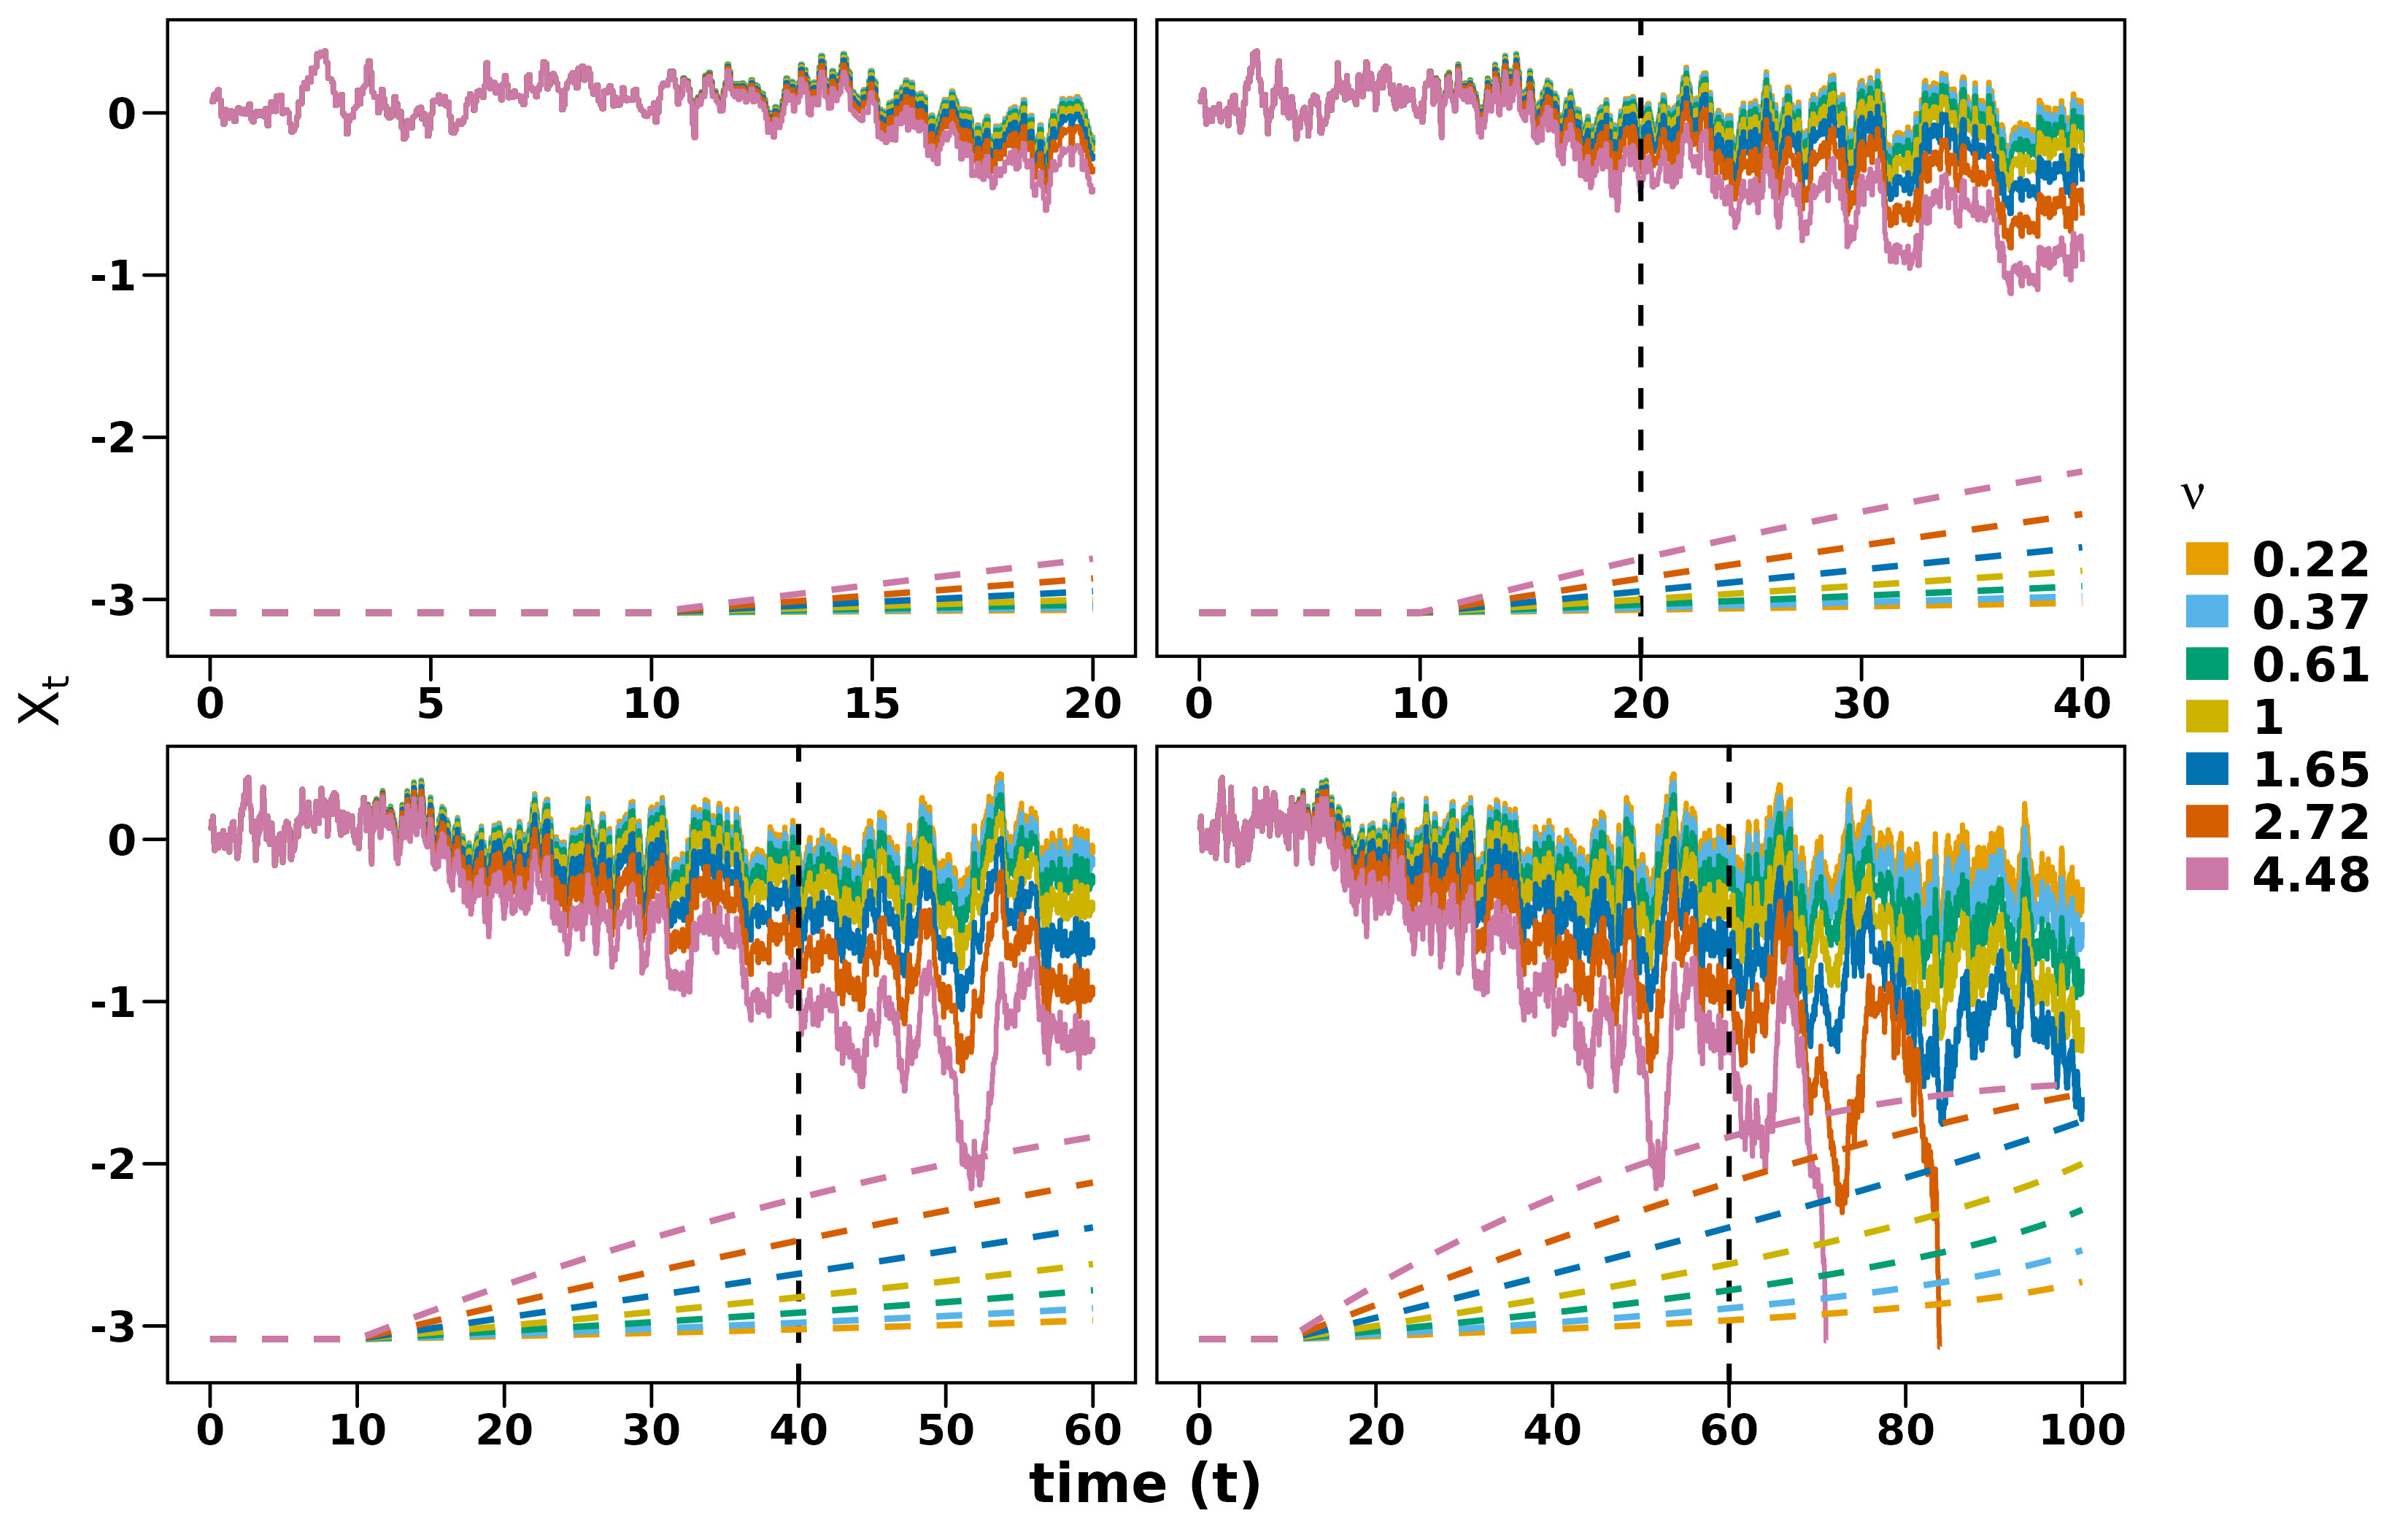
\includegraphics[scale = .13]{figures/mu_simulations_discussion_plot.jpeg}
    \caption{Sample paths for varying $\nu$ with the same realizations from the brownian motion cut at different points in time.}
    \label{figure:mu_simulations_discussion_plot}
    \end{center}
\end{figure}\\
This example is of course constructed for sake of illustration and the following points might not always hold. However, figure \ref{figure:mu_simulations_discussion_plot} is a clear example of some of the difficulties that can arise with regards to estimation of the $\nu$-parameter. In each facet the vertical dashed line marks the point in time upto which the facet before it ran. The colored dotted lines in the plots are the unstable fixed points that if crossed before the tipping point, most likely results in the process experiencing noise-induced tipping. This means that it will be too late to predict a tipping point from a saddle-node bifurcation, if we are relatively close to it. Furthermore, due to noise-tipping the process is no longer close to the stable fixed point, whence there is no information about $\nu$ from the samples anymore. Conversely, we need to have quite a long series of observations within the dynamic part of the process to be able to distinguish between the paths. With only $240$ observations within the dynamic part in the upper-left facet, we can barely tell sample paths coming from very different values of $\nu$ from one another, at least visually. However, as our experiments have shown estimating values even moderately far away from $\nu = 1$ results in difficulties for the optimizer. All in all we might need more sophisticated optimization methods than \code{optim} to have succes with estimating parameters such as $\nu$. This could be achieved how we have already discussed, while another option is using automatic differentiation lately made more easily applicable in \code{R} via the \code{torch} framework \cite{torch}, or even hand coding the optimizers. \\\\
Even another option is to develop the numerical optimizer even further, albeit its possibilites of finding fixed points for a range of values $t$ as required in the dynamical part are quite limited without some a priori given assumptions about the evolution of these fixed points. The strategy that might be applicable here is providing the specific form of $\lambda$ used throughout and use it to create sub-optimization problem. Though, we do not observe $\lambda$ directly, the sample paths should be close to the fixed point on average; assuming that the process does not tip due to noise, of course. With this we could perhaps use non-linear least squares to regress $\mu_t$ on the samples. We did experiment a bit with this with the method \code{stats::nls} but only got limited success. Solving the non-linear least squares at every iteration of the optimization is rather computationally expensive and it was quite error-prone: At some iterations the \code{stats::nls} failed due to other parameters such as $A$ making the problem infeasible. To avoid this we could for instance adopt the penalization of $A$ used in \cite{Ditlevsen2023}.\\
Another thing we tried was making the numerical Strang method purely numerical. That is, it should be implemented such that the user merely provides the data, the specific model one wants to fit and the usual values required for optimization. However, the user does not provide the lamperti SDE nor even the lamperti-transform (\ref{eq:lampertiDefinition}) here. To achieve this the method must construct these numerically, which we actually managed to do. Yet, the computational speed of the method became the bottleneck of development; it took too long to evaluate the likelihood even once for the method to ever be viable. Now, the raison d'être of the numerical methods are that they allow us to use the methods without going through extensive calculations. And while simplifying the calculations necessary down to nothing whatsoever would be nice, the method as is still provides a significant reduction in number of manual computations needed. Furthermore, it is uncertain if we would be able to match the results shown in figure \ref{figure:ARE_dist_linear_noise} or \ref{figure:ARE_dist_numeric_F_diffusion}, if we automated the calculations further. In addition, it is to be expected that a user wanting to apply these methods would be able to find the lamperti-transform and compute the lamperti SDE with Ito's formula, which is all the numerical Strang based method requires. This further cements keeping the numerical Strang method as it is. \\\\
We already touched on the idea of using the Strang splitting scheme to construct a score function. Now, a third way to use this scheme could be to construct martingale estimation equations for stochastic differential equations that are more complicated than the Pearson diffusions, e.g. the dynamic part of the process. As with our idea of using Kessler's method on the stochastic differential equation in the splitting, this method does not use the lamperti-transform of the process. To see this more easily, consider the square-root based dynamical part of the saddle-node normal form model
\begin{align}
    \mathrm{d}X_t = -(A(X_t - m)^2 + \lambda_t)\mathrm{d}t + \sigma\sqrt{X_t}\mathrm{d}W_t \label{eq:squareSplittingDiscussion}
\end{align}  
The following splitting is also in section \ref{subsubsec:squarerootDynamic}
\begin{align}
    \mathrm{d}X_t^{[1]} &= -\alpha(\lambda)\left(X_t^{[1]} - \mu(\lambda)\right)  \mathrm{d}t + \sigma \sqrt{X_t^{[1]}} \mathrm{d}W_t, \label{eq:squareRootSplit1_discussion} \\
    \mathrm{d}X_t^{[2]} &= - A \left(X_t^{[2]} - \mu(\lambda)\right)^2 \mathrm{d}t, \label{eq:squareRootSplit2_discussion}
\end{align}
with $\alpha(\lambda) = 2\sqrt{-A\lambda_t}$ and $\mu(\lambda) = m + \sqrt{-\frac{\lambda_t}{A}}$. As we mention in that part of the appendix this is applying the splitting heuristic from \cite{SplittingSchemes} to (\ref{eq:squareSplittingDiscussion}). However, what this gives us is an SDE (\ref{eq:squareRootSplit1_discussion}), for which we can construct martingale estimation equations. For the Strang composition, we recall that based on figure \ref{figure:StrangAndLieTrotterPlot} the flow is a non-linear transform of the solution to the SDE (\ref{eq:squareRootSplit1_discussion}). So constructing the estimation equations for the whole flow is a matter of using a result about the relationsship between eigenfunctions, $p_n(x)$ and eigenvalues $\lambda_n$ for a process such as $X_t^{[1]}$ and transformations of that process with functions such as $\varphi_2$. It turns out \cite[remark on p. 41]{StatisticalMethodsForSDE} that in this case the eigenfunctions are $p_n\left(\varphi_2^{-1}(x)\right)$ and the eigenvalues the same. Still, it is unlikely that we would be able to get the conditonal mean- and variance  of the flow from these eigenfunctions and eigenvalues, so in the remaining calculations one has to use a few more results from the theory of estimation equations than what have been presented here.
\subsection{Tipping of the AMOC}
Taking figure \ref{figure:surival_curve_taus} and table \ref{table:tipping_quantiles} as our starting points of the discussion, it is clear that all the models indicate tipping to be \textit{more} than likely within the next 140 years. By "likely" we understand the 66\% confidence interval that is used by the Intergovernmental Panel on Climate Change \cite{Ditlevsen2023}. Accross all models and fingerprints there is at least an $83.5\%$ chance of tipping occuring before the end of year $2169$; while what specifically is likely ranges a bit more according to the different models. Still, all the estimates from the data lie within medio 21st century and primo 22nd century. We did not investigate penalization on the models, but it would be interesting to adopt the penalization on $A$ into the $t$-diffusion based model as well. To get an idea of how this could affect the estimates of the tipping time consider pairs of estimates of tipping year and $A$ stratfied after model
\begin{figure}[h!]
    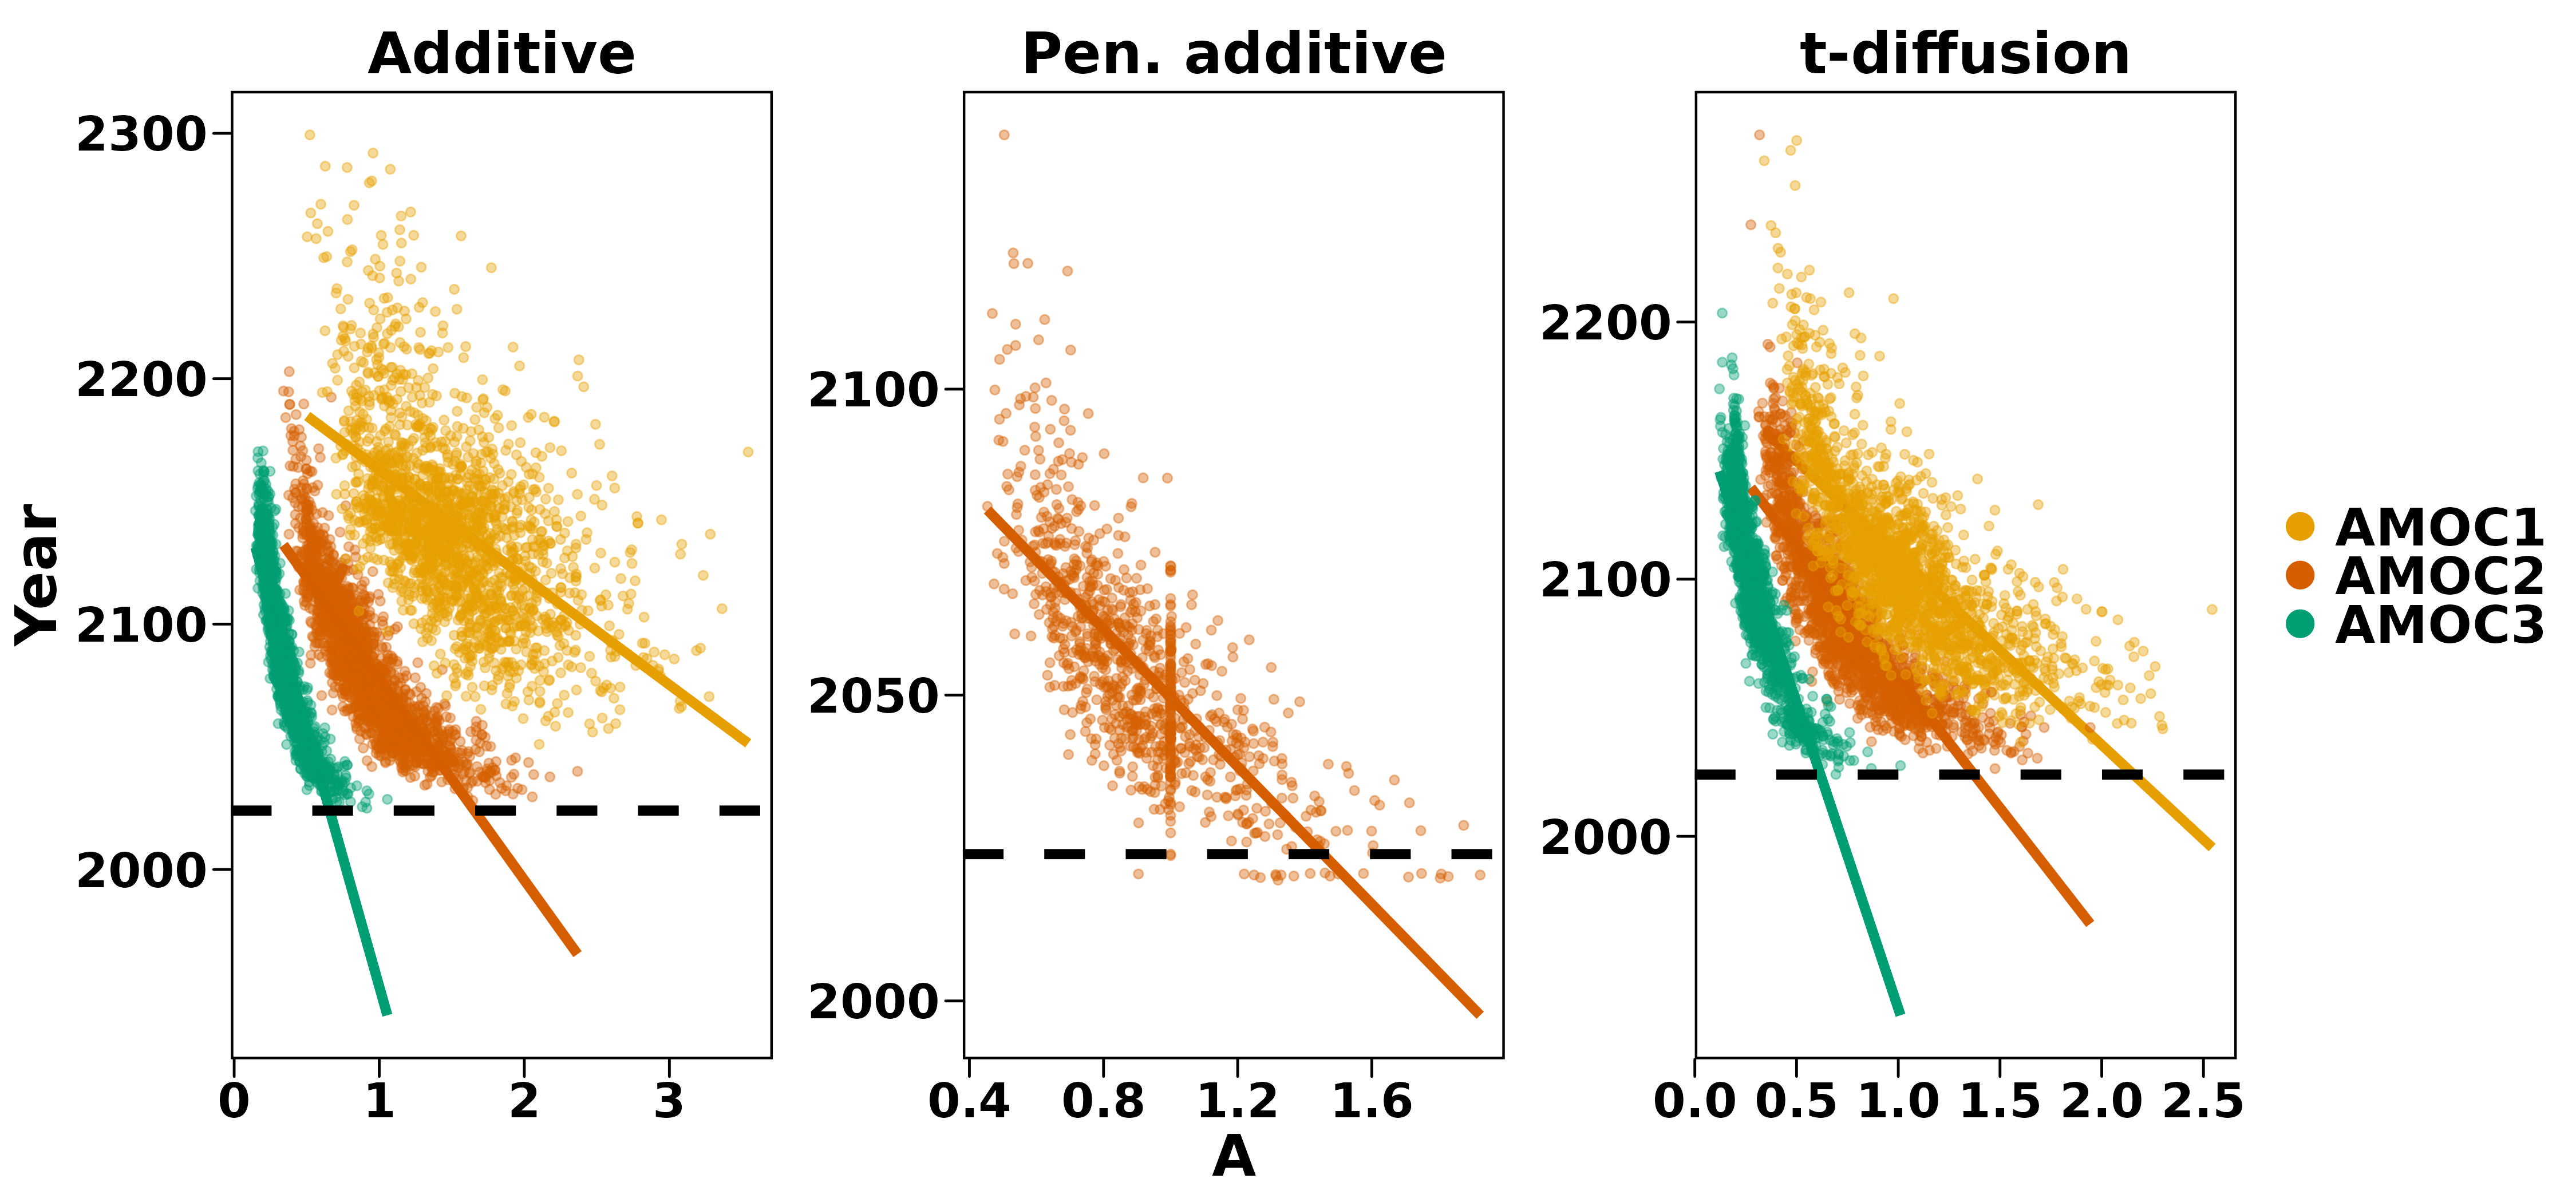
\includegraphics[scale = .095]{figures/correlation_between_A_and_tau_plot.jpeg}
    \caption{The graph shows pairs of estimates of tipping year and $A$ grouped by model and fingerprint type}
    \label{figure:correlation_A_and_tau}
\end{figure}\\
The lines in the graphs are linear normal models fitted to the stratified samples they share color and facet with. In all cases their is a clear negative correlation between the estimate of $A$ and -the tipping year; from the points in the graph it is clear that small values of $A$ tend to be paired with tipping estimates far in the future. Indicating that if we want to heavy-tailed estimators we might want to penalize values values of $A$ below 1 as done in the paper. However, as seen on the graph in figure \ref{figure:correlation_A_and_tau} this creates a clear bias towards $A = 1$. Actually, one could argue that the penalizations might hurt the optimization somewhat here. Note the clear vertical line forming around $A = 1$ in the middle graph of figure \ref{figure:correlation_A_and_tau}. This indicates that the optimization has a tendency to give estimates \textit{really} close to $A = 1$. In fact, a closer investigation reveals that penalization results in $12.5\%$ of estimates of $A$ being closer than $0.001$ units away from $1$. This is quite suspicious as this is practically one for floating point numbers; and this we get in 1 in 8 of the simulations. In addition, This limits the range of values of the tipping as well shifting $\tau$ in the specific direction shown by the negative correlation in figure \ref{figure:correlation_A_and_tau}. Now apart from this we also discovered a minor bug in the implementation of the dynamic OU likelihood function that is in the supplementary material of the paper resulting in the estimates shown being a bit different. Now, the bug has since been corrected and it has been checked that the distribution of the tipping time stays roughly the same after the fix, so the arguments and comparisons made with the paper here are still valid. Whence we do not redo all the computations to recreate the distributions of \cite{Ditlevsen2023}. Additionally, there are other slight differences in the choices made between the estimation methods of the paper and this project such as whether $\sigma$ or $\sigma^2$ is estimated etc. All these small differences can compound so the central estimate we quickly present here might not be the exact one, one would get with the corrected likelihood-implementation with the penalty. The tipping time estimate we get from the AMOC data with the penalized method and the exact penalization used there is 2055 for the AMOC2, which is rather close to the original result from the paper, confer table \ref{table:tipping_quantiles}.  
